\documentclass{article}
\usepackage{hyperref}
\usepackage{graphicx}
\usepackage{xcolor}

\title{MapReduce on GPU}
\author{Mark Doughten [md1875], \\ Abhilash Nambissan [ajn125], \\ Rishita Mane [rm1848]}
\date{April 27, 2025}

\begin{document}

\maketitle

\section{Technical Report}

This report outlines our project plan for implementing MapReduce with GPU integration to handle large workloads efficiently.

\subsection{Goal}
At the end of the semester, the team aims to demonstrate that combining MapReduce with GPU acceleration is beneficial, significantly reducing the runtime for certain operations such as word counting. We intend to design a system capable of distributed processing of compute jobs by splitting tasks and distributing them across CPUs and GPUs.

\begin{figure}[ht]
    \centering
    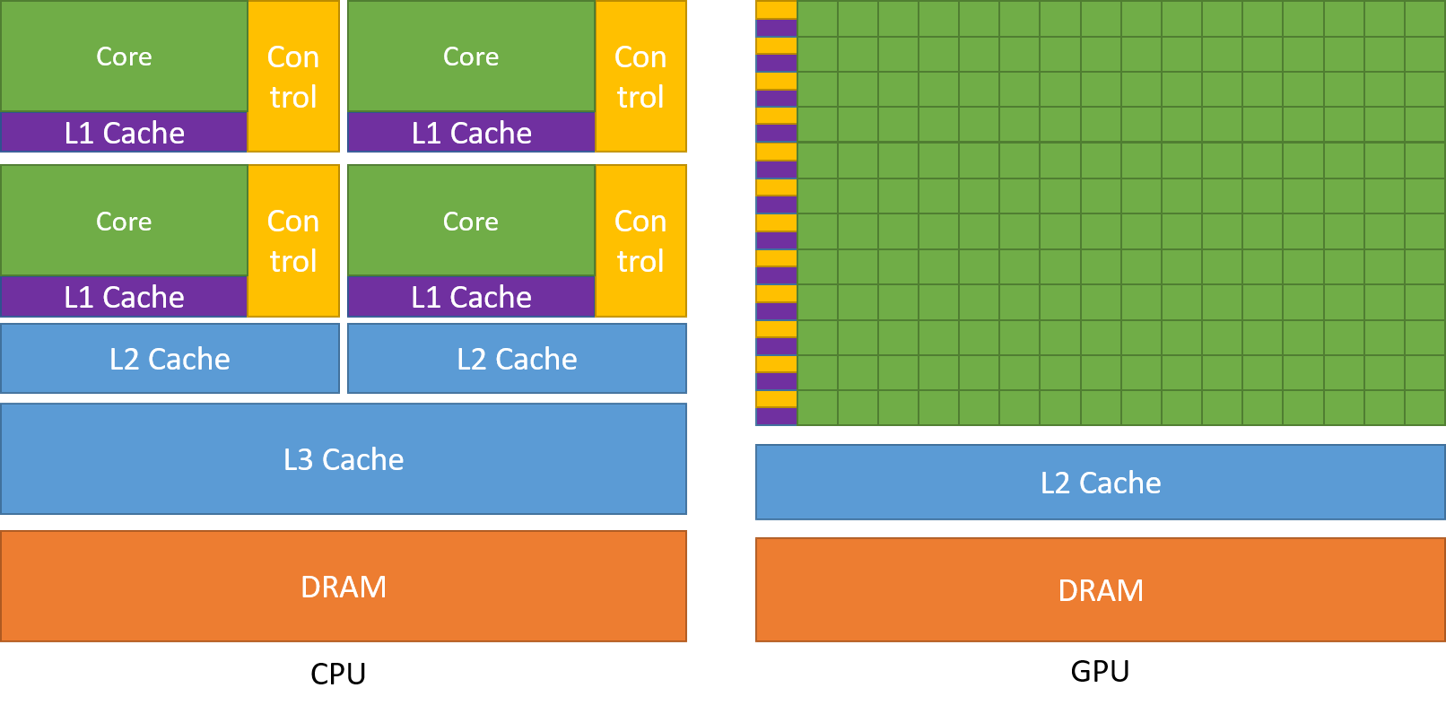
\includegraphics[width=.8\linewidth]{./images/chips.png}
    \caption{Chip Design \cite{cuda_docs}}
    \label{fig:mapreduce}
\end{figure}

\subsection{Description}
This work builds on the MapReduce framework originally designed at Google for clustering commodity hardware \cite{mapreduce}. Given the growing need for enhanced computing power in data processing and machine learning, we believe a framework that integrates MapReduce and GPU computing will improve system design by leveraging both commodity CPUs and specialized GPUs.

We will build upon the Mars framework \cite{mars}, a GPU-based MapReduce platform, and extend it to handle larger datasets exceeding device memory, using chunked processing and aggregation techniques.

\subsection{Control Flow}
The technical requirements include the CUDA programming language, designed for NVIDIA GPUs \cite{cuda_docs}. Our system will incorporate:
\begin{itemize}
    \item Host-side preprocessing to generate key-value pairs.
    \item Data transfer between CPU and GPU using pinned memory and asynchronous copies \cite{cuda_mem_pool}.
    \item Handling datasets larger than device memory via chunking and global aggregation.
    \item Two-stage MapReduce: \textit{(1) Chunk processing}, \textit{(2) Global aggregation.}
\end{itemize}

The combination of these features allows better memory management and throughput when operating on large datasets. The entire operation is completed in the Mars framework. 

\subsection{Memory Management Techniques}
Our project considers several memory management strategies to optimize data transfer between the CPU and GPU.

\begin{figure}[ht]
    \centering
    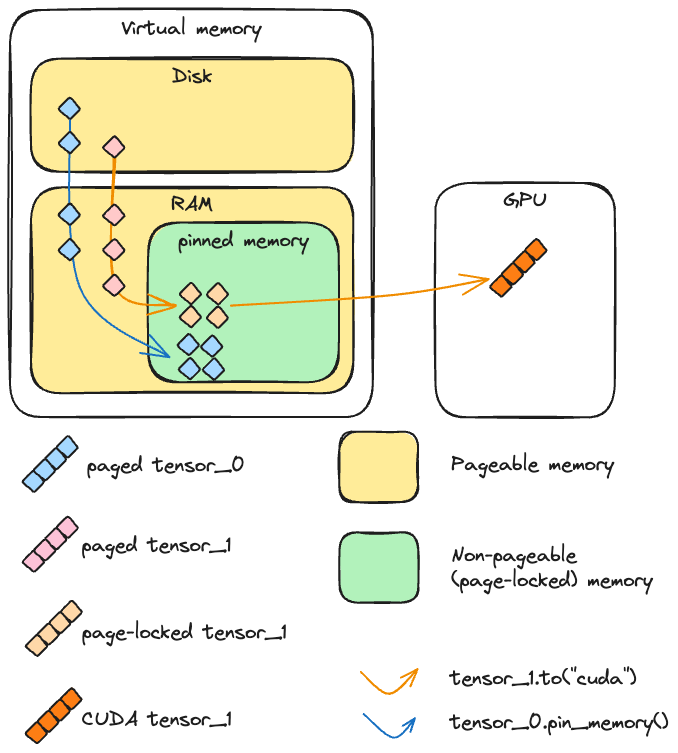
\includegraphics[width=.8\linewidth]{./images/pinmem.png}
    \caption{Pinned Memory \cite{pinned_memory}}
    \label{fig:mapreduce}
\end{figure}

\paragraph{Pageable Memory} Pageable (or non-pinned) memory is allocated using traditional system functions such as \texttt{malloc}. Transfers between pageable host memory and device memory use \texttt{cudaMemcpy} and are synchronous, meaning the CPU is blocked until the copy is complete. Pageable memory is managed by the operating system and can be paged out to disk, introducing transfer latency.

\paragraph{Pinned (Page-Locked) Memory} Pinned memory is allocated using \texttt{cudaMallocHost}, ensuring that the memory remains resident in physical RAM and is not swapped to disk. Pinned memory enables faster transfer speeds and allows for truly asynchronous memory copies using \texttt{cudaMemcpyAsync}. However, it consumes valuable physical memory and should be used selectively \cite{cuda_forum_async}.

\paragraph{Asynchronous Transfers} Asynchronous memory copies using \texttt{cudaMemcpyAsync} enable overlapping of data transfers and kernel execution, improving GPU utilization. Asynchronous copies require pinned memory to be effective and operate through CUDA streams, providing better concurrency between computation and communication.

\subsection{Chunking Strategies}
Our approach distinguishes between two types of chunking strategies depending on the dataset size.

\paragraph{Basic Chunking} The input dataset is divided into contiguous chunks that fit into device memory. Each chunk is processed sequentially: transfer from host to device, MapReduce execution, and result collection, using blocking memory copies.

\paragraph{Advanced Chunking with Async} For larger datasets, we implement an optimized chunking strategy:
\begin{itemize}
    \item Allocate pinned host memory and use asynchronous device memory pools \cite{cuda_mem_pool}.
    \item Utilize multiple CUDA streams to overlap data transfers and computation.
    \item Pipeline chunk loading, MapReduce execution, and output collection for maximum concurrency.
\end{itemize}

Our implementation supports both strategies, automatically selecting the advanced method when the dataset exceeds a configurable device memory threshold.

\begin{figure}[ht]
    \centering
    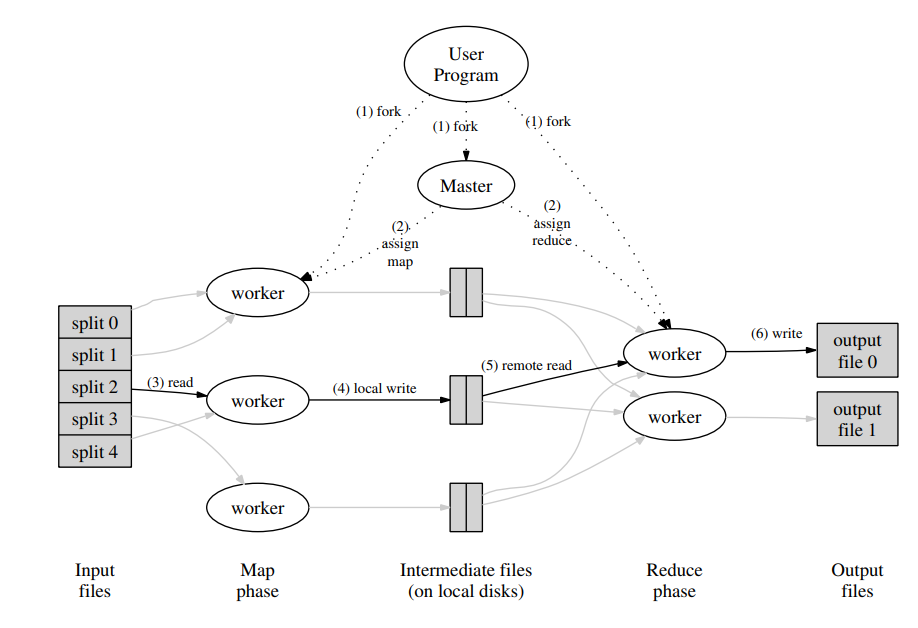
\includegraphics[width=1\linewidth]{./images/mapreduce.png}
    \caption{MapReduce Framework \cite{mapreduce}}
    \label{fig:mapreduce}
\end{figure}

\subsection{Measurements}
We will benchmark the performance of various workloads by measuring:
\begin{itemize}
    \item Throughput (operations per second)
    \item Per-operation latency
    \item Total job completion time
\end{itemize}

Comparisons will be made between CPU-only MapReduce and CPU+GPU hybrid execution.

\subsection{Risk Analysis}
A primary risk lies in hardware availability, particularly access to NVIDIA GPUs and environments supporting CUDA. Additionally, Mars and CUDA impose limitations on dynamic scheduling and memory management, which may impact large-scale experiments.

\section{Environment Configuration}

Our development environment is based on Docker containers running on Windows using WSL (Windows Subsystem for Linux) with GPU support. The setup process is outlined below:

\subsection{Windows Setup with WSL and Nvidia Container Toolkit}
\begin{itemize}
    \item Install WSL (Windows Subsystem for Linux) by following the instructions: \href{https://learn.microsoft.com/en-us/windows/wsl/setup/environment}{WSL Setup Guide}.
    \item Install Nvidia Container Toolkit to enable GPU access from within containers: \href{https://docs.nvidia.com/datacenter/cloud-native/container-toolkit/latest/install-guide.html}{Nvidia Container Toolkit Guide}.
    \item Verify the installation with the following command:
    \begin{verbatim}
    docker run --rm --gpus all nvidia/cuda:12.2.0-base-ubuntu22.04 nvidia-smi
    \end{verbatim}
\end{itemize}

\subsection{Container Setup}
We use a custom Docker container based on the CUDA 12.2 development image. The steps are:
\begin{itemize}
    \item Build the Docker image:
    \begin{verbatim}
    docker build -t cuda .
    \end{verbatim}
    \item Run the container with access to the GPUs and mount the project directory:
    \begin{verbatim}
    docker run --gpus all -it --rm -v $(pwd)/app:/app cuda bash
    \end{verbatim}
\end{itemize}

\subsection{Dockerfile Configuration}
The Dockerfile used for building the container:

\begin{verbatim}
FROM nvidia/cuda:12.2.0-devel-ubuntu22.04

ENV DEBIAN_FRONTEND=noninteractive

# Install system tools, Python, vim, and tmux
RUN apt-get update && \
    apt-get install -y \
    python3-pip \
    python3-dev \
    build-essential \
    git \
    curl \
    vim \
    tmux && \
    rm -rf /var/lib/apt/lists/*

# Upgrade pip and install core Python dependencies
RUN pip3 install --upgrade pip && \
    pip3 install cython numpy scipy cupy

# Set working directory
WORKDIR /app

# Default command to keep container running
CMD ["tail", "-f", "/dev/null"]
\end{verbatim}

This container includes all the necessary dependencies for our project, including CUDA development libraries, Python libraries for numerical computing, and common tools like \texttt{vim} and \texttt{tmux} for in-container development.



\section{Responses to Technical Questions}

\subsection{Programming Specification}
We plan to leverage the Mars API \cite{mars} for basic MapReduce operations. Mars abstracts the map, group, and reduce phases in CUDA kernels. Initially, we will use the Mars API as-is, and later experiment with large dataset support and dynamic load balancing improvements. Although dynamic scheduling across threads is limited on current GPUs \cite{dynamic_scheduling}, Mars handles load balancing reasonably well at the value list level.

\subsection{Decomposition Across CPU and GPU}
Data processing is decomposed as follows:
\begin{itemize}
    \item \textbf{CPU}: File I/O, preprocessing into key-value pairs.
    \item \textbf{GPU}: Execution of map, group, and reduce stages.
\end{itemize}

For large datasets exceeding device memory, our framework implements:
\begin{itemize}
    \item Chunked processing: breaking data into manageable chunks.
    \item Memory pool management: optimizing asynchronous device memory usage.
    \item Two-stage MapReduce: post-processing chunk outputs into a global aggregation.
\end{itemize}

\subsection{Existing Frameworks and Novelty}
Mars is an existing MapReduce framework for GPUs \cite{mars}. Our framework differs in the following ways:
\begin{itemize}
    \item Handling datasets larger than GPU memory through chunking.
    \item Integrating memory pool optimizations and CUDA asynchronous streams.
    \item Performing a second MapReduce stage for global aggregation.
\end{itemize}

This makes our system closer to production-grade MapReduce frameworks capable of scaling beyond individual device limitations.

\section{References}
\begin{thebibliography}
\raggedright

\bibitem{mapreduce}
J. Dean and S. Ghemawat, \textit{MapReduce: Simplified Data Processing on Large Clusters}. \href{https://dl.acm.org/doi/10.1145/1327452.1327492}{https://dl.acm.org/doi/10.1145/1327452.1327492}

\bibitem{mars}
B. He, W. Fang, Q. Luo, N. Govindaraju, and T. Wang, \textit{Mars: A MapReduce Framework on Graphics Processors}. \href{https://dl.acm.org/doi/10.1145/1454115.1454152}{https://dl.acm.org/doi/10.1145/1454115.1454152}

\bibitem{cuda_docs}
NVIDIA, \textit{CUDA C Programming Guide}. \href{https://docs.nvidia.com/cuda/cuda-c-programming-guide/contents.html}{https://docs.nvidia.com/cuda/cuda-c-programming-guide/contents.html}

\bibitem{cuda_mem_pool}
NVIDIA, \textit{CUDA Memory Pools API}. \href{https://docs.nvidia.com/cuda/cuda-runtime-api/group__CUDART__MEMORY__POOLS.html}{https://docs.nvidia.com/cuda/cuda-runtime-api/group\_\_CUDART\_\_MEMORY\_\_POOLS.html}

\bibitem{cuda_forum_async}
NVIDIA Developer Forum, \textit{Confusion about Synchronization and cudaMemcpyAsync}. \href{https://forums.developer.nvidia.com/t/confusion-about-synchronization-or-asynchronization-of-cudamemcpy-and-cudamemcpyasync/276826/4}{https://forums.developer.nvidia.com/t/confusion-about-synchronization-or-asynchronization-of-cudamemcpy-and-cudamemcpyasync/276826/4}

\bibitem{dynamic_scheduling}
M. Steinberger, \textit{On Dynamic Scheduling for GPUs}. \href{https://www.markussteinberger.net/papers/OnDynamicScheduling.pdf}{https://www.markussteinberger.net/papers/OnDynamicScheduling.pdf}

\bibitem{pinned_memory}
A guide on good usage of non\_blocking and pin\_memory() in PyTorch. \href{https://pytorch.org/tutorials/intermediate/pinmem_nonblock.html}{https://pytorch.org/tutorials/intermediate/pinmem\_nonblock.html}


\end{thebibliography}

\end{document}